%encoding UTF-8
\author{Евгений Синельников, Игорь Чудов}
\city{Саратов}
\affiliation{Базальт СПО}
\projecttitle{ALT Join}
\projecturl{\url{http://altlinux.org/}}
\title{Приобщение к участию в разработке свбодных программ на примере
стажировки в компании Базальт СПО}
\maketitle

\begin{abstract}
  В рамках доклада рассмотрена проблема обучения новых
  сотрудников в компаниях, работающих с СПО. Предложены методики для
  ускорения процедуры включения людей в рабочие процессы. Представлены
  примеры вводных документов.
\end{abstract}


\section{Проблематика}

В сравнении с компаниями, ориентированными на outsource-разработку для
множества различных заказчиков, небольшие продуктовые компании
испытывают дефицит кадров.

В качестве примера предлагается рассмотреть выборку заявок на Join
с сайта \url{http://bugzilla.altlinux.org/} за весь доступный период
(2008-2020 годы):

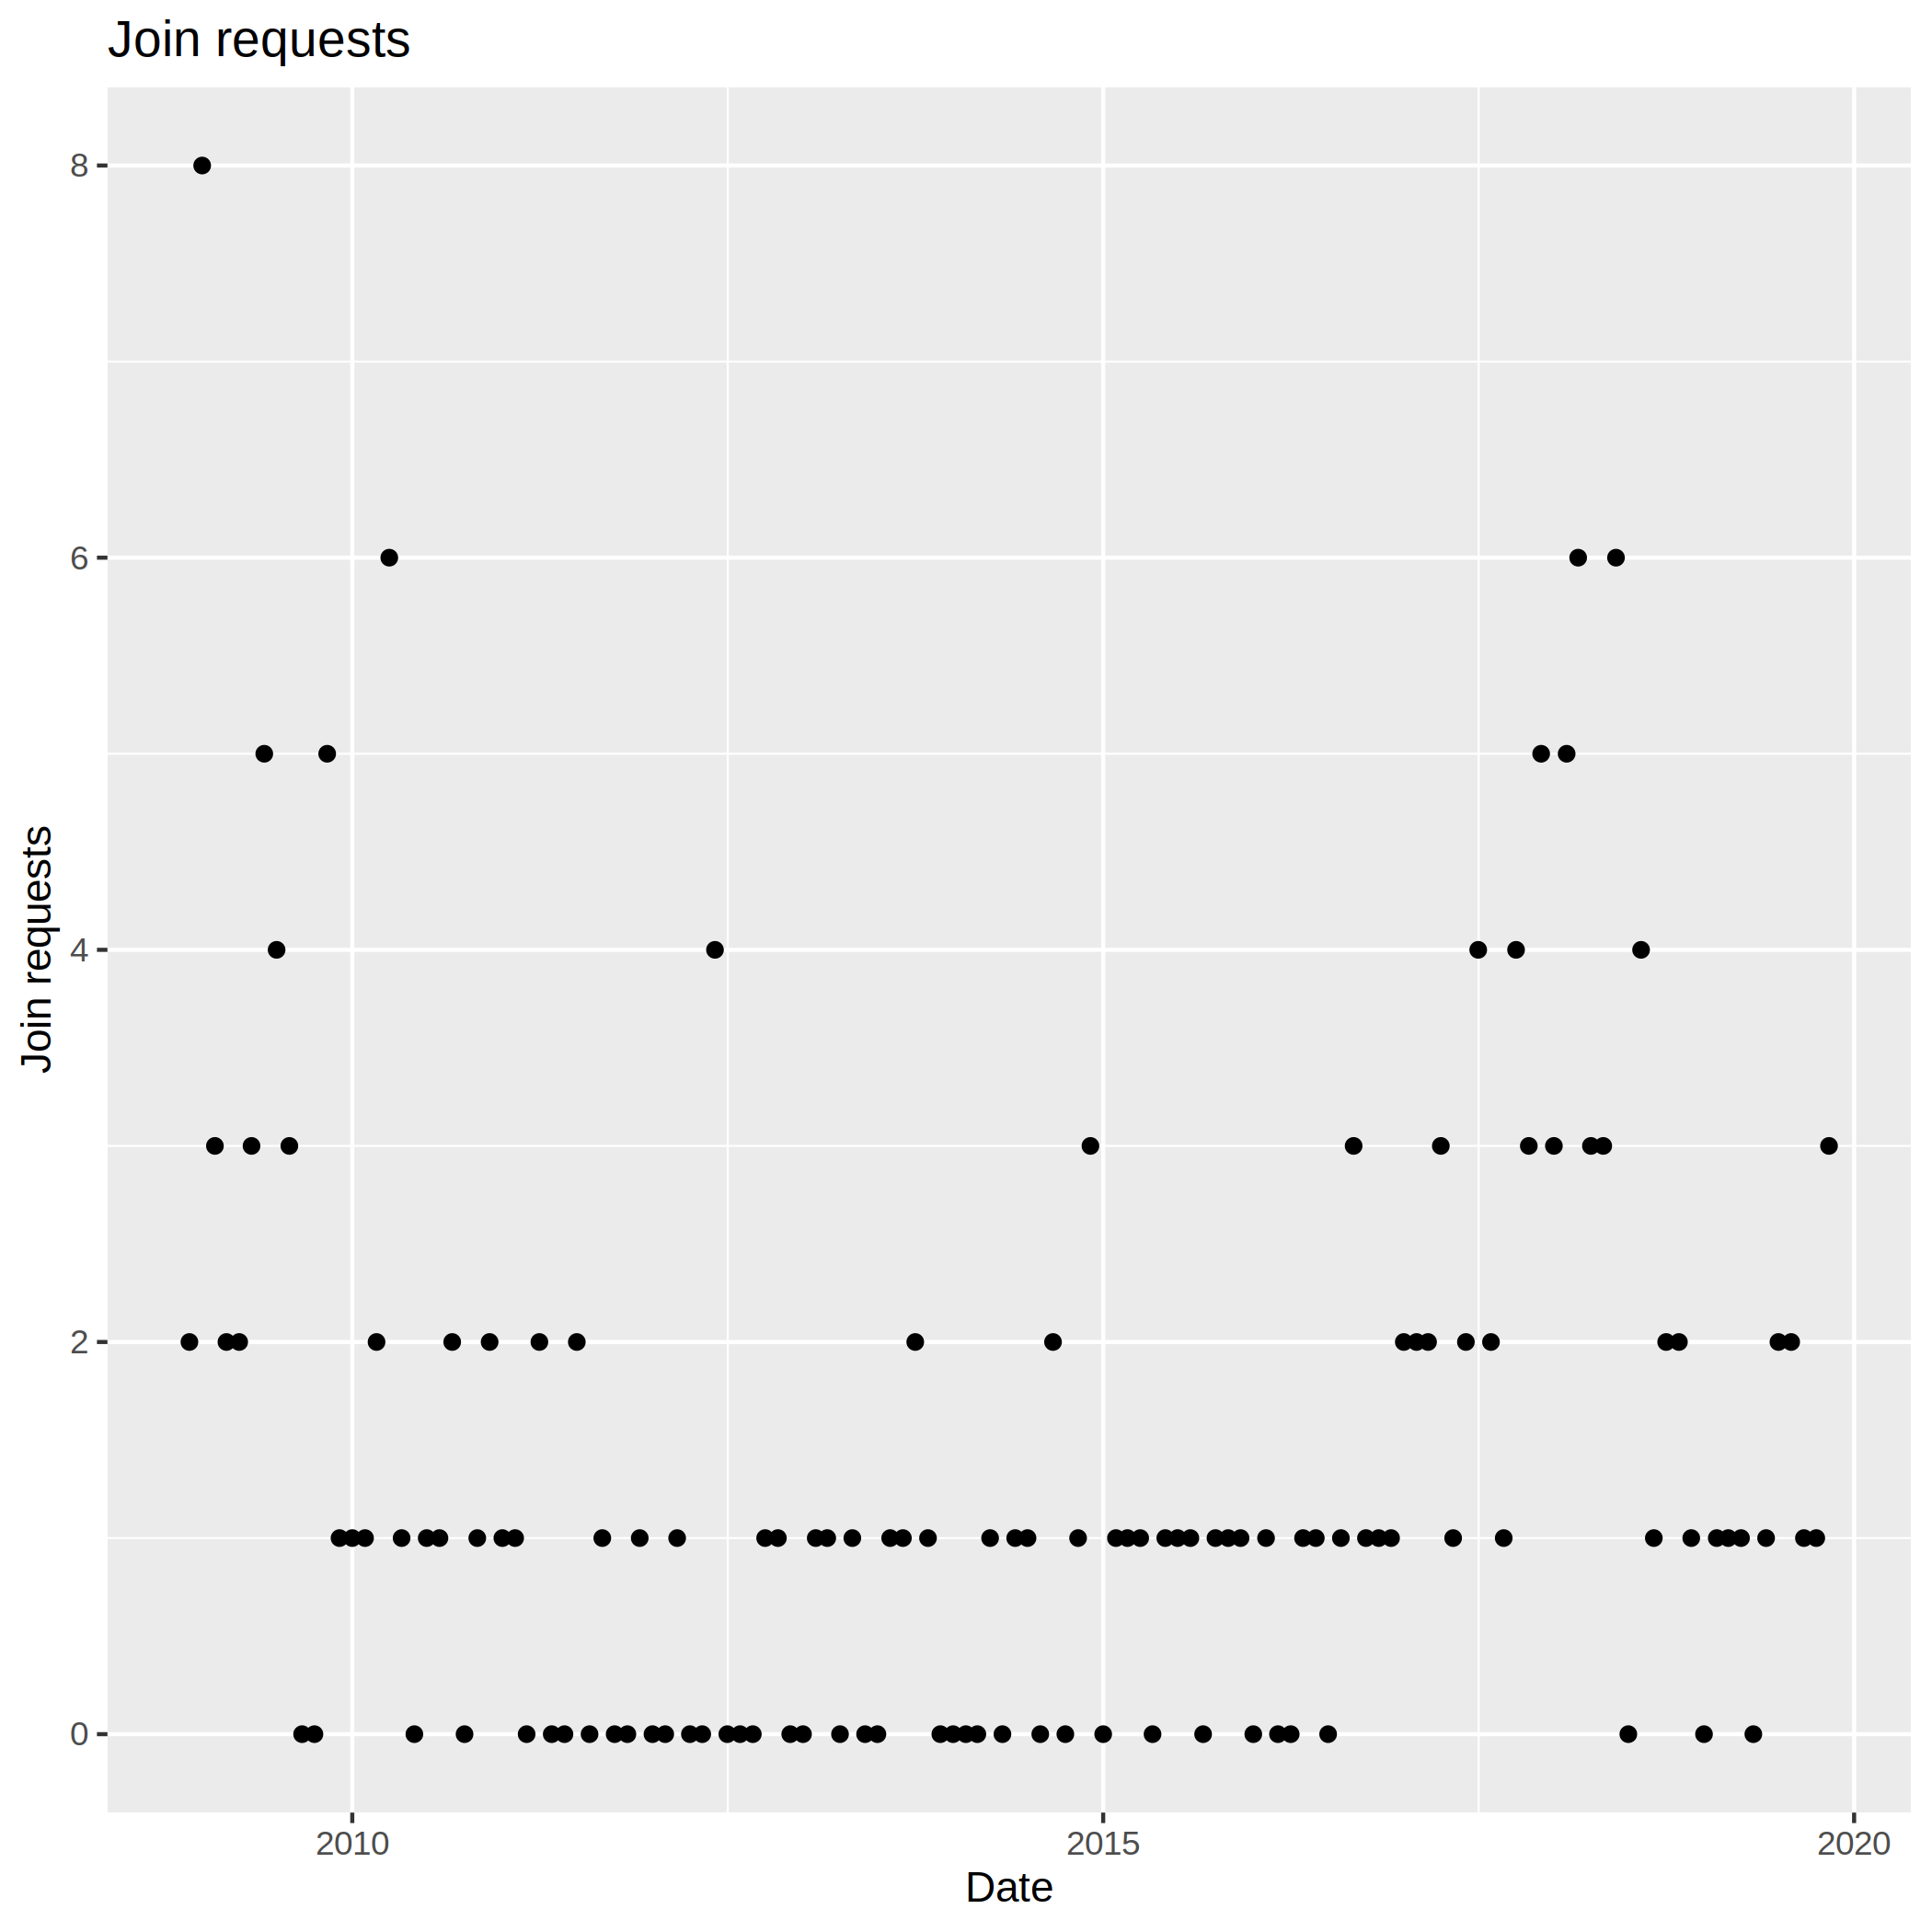
\includegraphics[width=\textwidth,height=\textheight,keepaspectratio]{ggplot}

Данные представляют из себя формальную характеристику потока
потенциальных сотрудников. Не смотря на длительный период выборки можно
отметить, что количество поступающих заявок невелико, что может служить
сигналом о нескольких проблемах:

\begin{itemize}
\item Проблема с процедурой подачи заявок (неочевидность, сложность,
бюрократия, длительность).
\item Проблема с методом коммуникации (устаревание инструмента и
методики, недостаточность усилий по преодолению барьеров коммуникации).
\item Также сказывается специфика предметной области с которой связана
работа.
\end{itemize}

Поступающие кадры незнакомы с базовыми понятиями отрасли, также не
воспринимают принятые в сообществе разработчиков СПО средства
коммуникации.

Для участия в стажёрской программе была размещена заявка на HeadHunter
со следующими результатами:

\begin{itemize}
\item 28 входящих заявок получено;
\item из них 6 человек отправили свои резюме и пришли на собеседование;
\item из 6 человек было отобрано 4 стажёра;
\item один стажёр отказался от работы через 4 дня.
\end{itemize}


\section{Методы решения проблемы}

Для ускорения процедуры адаптации сотрудников были опробованы следующие
методы:

\begin{itemize}
\item Раздаточные материалы: одностраничная брошюра с базовыми ссылками и
программами, на которой сотрудник может сделать пометки.
\item Коллективно дополняемая публичная документация и статьи.
\item Менторинг.
\end{itemize}

Предложенные методы были опробованы в рамках стажёрской программы
компании "Базальт СПО". Совершена попытка ускорить процесс адаптации
новых сотрудников. Для этого в первый рабочий день для коллектива
стажёров была проведена вводная лекция и передана "раздатка" -
одностраничная памятка с целями сотрудника на рабочий период, ссылками
на основные ресурсы Интернет и кратким описанием требуемых программ. Это
позволило людям лучше запоминать основы за счёт возможности сделать
записи на раздаточном материале.


\section{Анализ результатов}

В рамках месячной стажировки получены следующие результаты:

\begin{itemize}
\item Один из стажёров разработал утилиту ALT Media Writer дополнив и
улучшив один из открытых проектов.
\item Второй стажёр занимался тестированием Samba и в результате сильно
продвинул проект разбирая большое количество use-cases.
\item Третий стажёр занимался написанием документации к Samba на публичной
Wiki \url{http://www.altlinux.org/}. В результате он получил как
общее понимание проекта, так и сделал его доступнее для русскоязычных 
пользователей.
\end{itemize}

На основании полученных результатов сделаны выводы:

\begin{itemize}
\item Специфика отрасли требует найма сотрудников и стажёров высокой
квалификации;
\item Приходящие с рынка кадры в большинстве своём недообучены и
обладают недостаточной квалификацией;
\item Работа со стажёрами недостаточной квалификации забирает
непозволительно много времени у основного состава сотрудников, что
понижает рентабельность найма стажёров;
\end{itemize}


\section{Библиография}

\begin{thebibliography}{9}
\bibitem{altbug} ALT Linux Bugzilla \url{http://bugzilla.altlinux.org/}
\bibitem{altwiki} ALT Linux Wiki \url{http://www.altlinux.org/}
\end{thebibliography}


%%% Local Variables: 
%%% mode: latex
%%% TeX-master: "../main"
%%% End: 
